\documentclass[11pt]{article}

\usepackage[T1]{fontenc}
\usepackage[utf8]{inputenc}

\PassOptionsToPackage{hyphens}{url}
\usepackage[
colorlinks=true,linkcolor=blue,urlcolor=blue,citecolor=blue,bookmarks=true,
bookmarksopenlevel=2]{hyperref}
\usepackage{amsmath,amssymb,amsthm,textcomp}
\usepackage{tikz}
\usepackage{cleveref}

\usepackage{minted}
\definecolor{gray}{rgb}{0.85,0.85,0.85}
\setminted[bash]{bgcolor=gray}
\setminted[python]{breaklines}

\usepackage{graphicx}

\usepackage{geometry}
\geometry{%total={210mm,297mm},
left=25mm,right=25mm,%
bindingoffset=0mm, top=20mm,bottom=20mm}

\setlength\parindent{0pt}
\setlength{\parskip}{1mm}

\sloppy

\title{Sample Solutions}
\author{Wolfgang Hönig\footnote{Now at California Institute of Technology}, Jiaoyang Li, Sven Koenig --- University of Southern California}
\date{Model AI Assignments 2020: Project on Multi-Agent Path Finding (MAPF)}

\begin{document}
\maketitle

\section{Task 1: Implementing Space-Time A*}

\subsection{Searching in the Space-Time Domain}

Changed lines (with respect to the student-provided code) are highlighted below:

\begin{minted}[highlightlines={1,3,8,16,17,18,20,23}]{python}
root = {'loc': start_loc, 'g_val': 0, 'h_val': h_value, 'parent': None, 'timestep': 0}
push_node(open_list, root)
closed_list[(root['loc'], root['timestep'])] = root
while len(open_list) > 0:
    curr = pop_node(open_list)
    if curr['loc'] == goal_loc:
        return get_path(curr)
    for dir in range(5):
        child_loc = move(curr['loc'], dir)
        if my_map[child_loc[0]][child_loc[1]]:
            continue
        child = {'loc': child_loc,
                'g_val': curr['g_val'] + 1,
                'h_val': h_values[child_loc],
                'parent': curr,
                'timestep': curr['timestep'] + 1}
        if (child['loc'], child['timestep']) in closed_list:
            existing_node = closed_list[(child['loc'], child['timestep'])]
            if compare_nodes(child, existing_node):
                closed_list[(child['loc'], child['timestep'])] = child
                push_node(open_list, child)
        else:
            closed_list[(child['loc'], child['timestep'])] = child
            push_node(open_list, child)
\end{minted}

\begin{minted}[highlightlines={2}]{python}
def move(loc, dir):
    directions = [(0, -1), (1, 0), (0, 1), (-1, 0), (0, 0)]
    return loc[0] + directions[dir][0], loc[1] + directions[dir][1]
\end{minted}

\subsection{Handling Vertex Constraints and Adding Edge Constraints}

In \texttt{a\_star}:
\begin{minted}{python}
constraint_table = build_constraint_table(constraints, agent)
# ...
        if my_map[child_loc[0]][child_loc[1]] or is_constrained(curr['loc'], child_loc, curr['timestep'] + 1,
                                                              constraint_table):
            continue
\end{minted}

Helper functions:

\begin{minted}{python}
def build_constraint_table(constraints, agent):
    max_timestep = -1  # the maximum timestep in these constraints
    for constraint in constraints:
        if constraint['agent'] == agent:
            max_timestep = max(max_timestep, constraint['timestep'])

    constraint_table = [[] for _ in range(max_timestep + 1)]

    for constraint in constraints:
        if constraint['agent'] == agent:
            constraint_table[constraint['timestep']].append({'loc': constraint['loc']})

    return constraint_table


def is_constrained(curr_loc, next_loc, next_time, constraint_table):
    if len(constraint_table) <= next_time:
        return False

    for constraint in constraint_table[next_time]:
        if constraint['loc'] == [next_loc] or constraint['loc'] == [curr_loc, next_loc]:
                return True 

    return False
\end{minted}


\subsection{Handling Goal Constraints}

The new constraint is violated without an additional goal test condition (that is, agent 0 will be at the goal location at timestep 10). One possible goal test condition is the following:

\begin{minted}{python}
if curr['loc'] == goal_loc:
    found = True
    if curr['timestep'] + 1 < len(constraint_table):
        for t in range(curr['timestep'] + 1, len(constraint_table)):
            if is_constrained(goal_loc, goal_loc, t, constraint_table):
                found = False
                break
    if found:
        return get_path(curr)
\end{minted}

\subsection{Optional: Designing Constraints}

\begin{itemize}
    \item One possible set of constraints is the following:
\begin{minted}{python}
        constraints = [
            {'agent' : 1, 'loc': [(1,4)], 'timestep': 2},
            {'agent' : 1, 'loc': [(1,3)], 'timestep': 2},
            {'agent' : 1, 'loc': [(1,2)], 'timestep': 2}
        ]
\end{minted}
    \item Output paths: [[(1, 1), (1, 2), (1, 3), (1, 4), (1, 5)], [(1, 2), (1, 3), (2, 3), (1, 3), (1, 4)]]
    \item Sum of costs: 8
\end{itemize}

\section{Task 2: Implementing Prioritized Planning}

\subsection{Adding Vertex Constraints}

(See solution below.)

\subsection{Adding Edge Constraints}

\begin{minted}{python}
for t in range(len(path)):
    for k in range(i, self.num_of_agents):
        # add vertex constraint
        constraints.append({'agent': k,
                            'loc': [path[t]],
                            'timestep': t})
        # add edge constraint
        if t > 0:
            constraints.append({'agent': k,
                                'loc': [path[t], path[t - 1]],
                                'timestep': t})
\end{minted}

\subsection{Optional: Adding Additional Constraints}

Here, we use a a global constraint set and after finding a path for an agent, we add constraints extracted from that path to all future agents. The following is executed after calling \mintinline{python}{a_star}:

\begin{minted}{python}
for t in range(len(path), upper_bound+1):
    for k in range(i, self.num_of_agents):
        # add vertex constraint
        constraints.append({'agent': k,
                            'loc': [path[-1]],
                            'timestep': t})
\end{minted}

\mintinline{python}{upper_bound} is a very large number or (better) computed as in the next task assignment.

\subsection{Optional: Addressing Failures}

A good upper bound for the path length is $height \cdot width \cdot \mbox{\it longest possible path length}$:

\begin{minted}[highlightlines={1,4,7,10}]{python}
max_path_length = 0

for i in range(self.num_of_agents):  # Find path for each agent
    upper_bound = len(self.my_map) * len(self.my_map[0]) + max_path_length
    path = a_star(self.my_map, self.starts[i], self.goals[i], self.heuristics[i],
                  i, constraints)
    if path is None or len(path)>=upper_bound:
        raise BaseException('No solutions')
    result.append(path)
    max_path_length = max(max_path_length, len(path))
\end{minted}

\subsection{Optional: Showing that Prioritized Planning is Incomplete and Suboptimal}

\begin{itemize}

\item Design a MAPF instance for which prioritized planning does not find an (optimal or suboptimal) collision-free solution for a given ordering of the agents. 

\textbf{Example}: Agent 1 moves from A to C, and agent 2 moves from B to D. 
\begin{center}
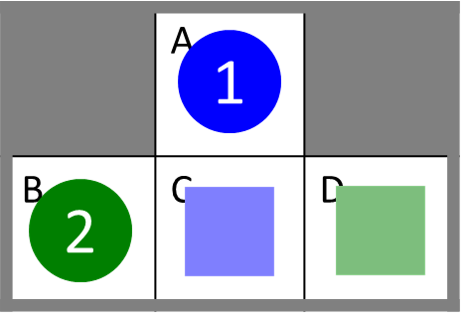
\includegraphics[width=0.18\textwidth]{images/sol1.png}
\end{center}
If agent 1 has higher priority than agent 2, then prioritized planning does not find an (optimal or suboptimal) collision-free solution because it first finds path [A, C] for agent 1 and then fails to find any collision-free path for agent 2. 

\item Design a MAPF instance for which prioritized planning does not find an (optimal or suboptimal) collision-free solution, no matter which ordering of the agents it uses. 

\textbf{Example}: Agent 1 moves from C to F, and agent 2 moves from E to B. 
\begin{center}
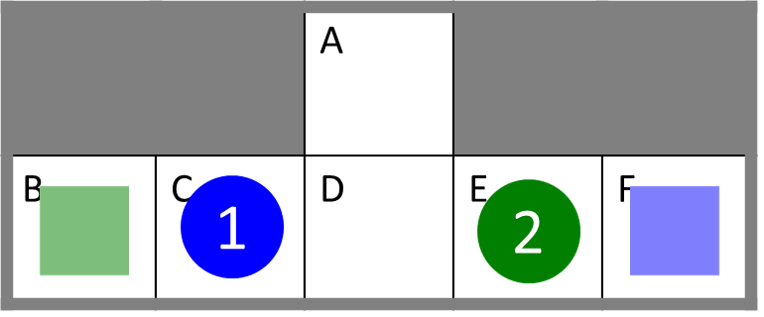
\includegraphics[width=0.30\textwidth]{images/sol2.png}
\end{center}

If agent 1 has higher priority than agent 2, then prioritized planning first finds path [C, D, E, F] for agent 1 and then fails to find any collision-free path for agent 2. If agent 2 has higher priority than agent 1, then prioritized planning first finds path [E, D, C, B] for agent 2 and then fails to find any collision-free path for agent 1.

\item Design a MAPF instance for which prioritized planning does not find an (optimal or suboptimal) collision-free solution for a given ordering of the agents even if an ordering of the agents exists for which prioritized planning finds an optimal collision-free solution. 

\textbf{Example}: Agent 1 moves from A to C, and agent 2 moves from B to D. 
\begin{center}
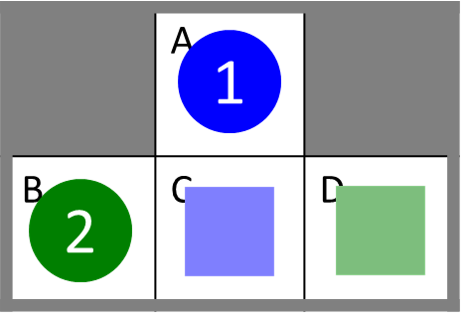
\includegraphics[width=0.18\textwidth]{images/sol1.png}
\end{center}
If agent 1 has higher priority than agent 2, then prioritized planning does not find an (optimal or suboptimal) collision-free solution because it first finds path [A, C] for agent 1 and then fails to find any collision-free path for agent 2. However, if agent 2 has higher priority than agent 1, then prioritized planning finds the optimal collision-free solution (of cost 4), which consists of path [A, A, C] (of length 2) for agent 1 and path [B, C, D] (of length 2) for agent 2. 

\item Design a MAPF instance for which prioritized planning finds a suboptimal (but not optimal) collision-free solution for a given ordering of the agents even if an ordering of the agents exists for which prioritized planning finds an optimal collision-free solution. 

\textbf{Example}: Agent 1 moves from D to H, and agent 2 moves from G to C. 
\begin{center}
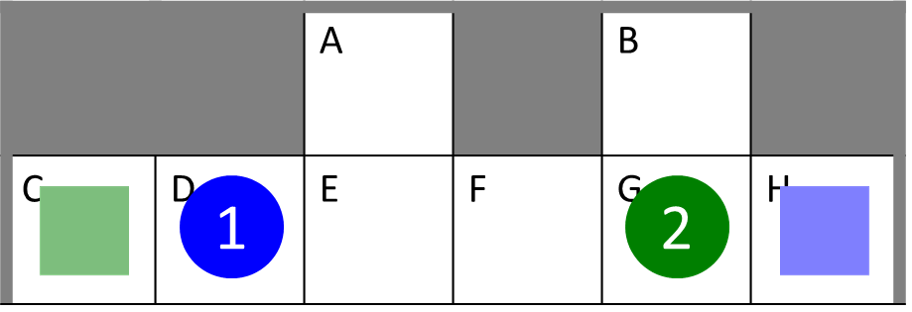
\includegraphics[width=0.36\textwidth]{images/sol4.png}
\end{center}

If agent 1 has higher priority than agent 2, then prioritized planning finds a suboptimal collision-free solution (of cost 12) that consists of path [D, E, F, G, H] (of length 4) for agent 1 and path [G, B, B, B, G, F, E, D, C] (of length 8) for agent 2. However, if agent 2 has higher priority than agent 1, then prioritized planning is able to find the optimal collision-free solution (of cost 10), which consists of path [D, E, A, E, F, G, H] (of length 6) for agent 1 and path [G, F, E, D, C] (of length 4) for agent 2. 

\item Design a MAPF instance for which prioritized planning does not find an optimal collision-free solution, no matter which ordering of the agents it uses, even if a collision-free solution exists.

\textbf{Example}: Agent 1 moves from E to J, and agent 2 moves from I to D. 
\begin{center}
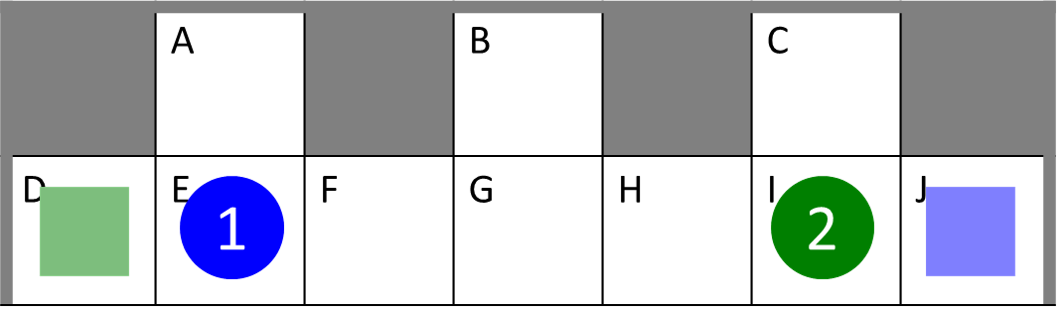
\includegraphics[width=0.42\textwidth]{images/sol5.png}
\end{center}

If agent 1 has higher priority than agent 2, then prioritized planning finds a suboptimal collision-free solution (of cost 15) that consists of path [E, F, G, H, I, J] (of length 5) for agent 1 and path [I, C, C, C, C, I, H, G, F, E, D] (of length 10) for agent 2. If agent 2 has higher priority than agent 1, then prioritized planning finds a suboptimal collision-free solution (of cost 15) that consists of path [E, A, A, A, A, E, F, G, H, I, J] (of length 10) for agent 1 and path [I, H, G, F, E, D] (of length 5) for agent 2. However, the optimal collision-free solution is of cost 13 and consists of path [E, F, G, B, G, H, I, J] (of length 7) for agent 1 and path [I, H, H, G, F, E, D] (of length 6) for agent 2. 

\end{itemize}

\section{Task 3: Implementing Conflict-Based Search (CBS)}

\subsection{Detecting Collisions}

\begin{minted}{python}
def detect_collision(path1, path2):
    for t in range(max(len(path1), len(path2))):
        # extract the current coordinates along the path
        c1 = get_location(path1, t)
        c2 = get_location(path2, t)
        if c1 == c2:
            return [c1, t]
        else:
            # extract the previous coordinates along the path
            # (for edge checking)
            p1 = get_location(path1, t - 1)
            p2 = get_location(path2, t - 1)
            if c1 == p2 and c2 == p1:
                return [p1, c1, t]
    return None
    
def detect_collisions(paths):
    collisions = []
    for i in range(len(paths) - 1):
        for j in range(i + 1, len(paths)):
            collision = detect_collision(paths[i], paths[j])
            if collision is not None:
                collisions.append({'a1': i,
                                  'a2': j,
                                  'loc': collision[:-1],
                                  'timestep': collision[-1]})
    return collisions
\end{minted}

\subsection{Converting Collisions to Constraints}

\begin{minted}{python}
def standard_splitting(collision):
    constraint1 = {'agent': collision['a1'],
                   'loc': collision['loc'],
                   'timestep': collision['timestep'],
                   'positive': False}
    loc = list(collision['loc'])
    loc.reverse()  # if this is an edge collision, we need to use
                   # the other direction of the edge in the constraint
    constraint2 = {'agent': collision['a2'],
                   'loc': loc,
                   'timestep': collision['timestep'],
                   'positive': False}
    return [constraint1, constraint2]
\end{minted}

\subsection{Implementing the High-Level Search}

\begin{minted}{python}
# Search the tree until the open list is empty
while len(self.open_list) > 0:

    node = self.pop_node()  # pop the node with the minimum cost
    if node['collisions'] == []:  # the paths of this node is collision-free
        self.print_results(node)
        return node['paths']

    collision = node['collisions'][0]  # choose a collision
    print("Choose a collision between {} and {} at location {} at timestep {}".format(
        collision['a1'], collision['a2'], collision['loc'], collision['timestep']))

    # Generate constraints to resolve the chosen collision
    new_constraints = standard_splitting(collision)

    for constraint in new_constraints:  # for each constraint, generate a child node
        i = constraint['agent']
        print("Negative constraint on agent {} at location {} at timestep {}".format(
                constraint['agent'], constraint['loc'], constraint['timestep']))

        constraints = list(node['constraints'])  # copy constraints
        constraints.append(constraint)  # add additional constraint

        paths = list(node['paths'])  # copy paths
        paths[i] = a_star(self.my_map, self.starts[i], self.goals[i], self.heuristics[i],
                          i, constraints)  # replan for this agent

        # Generate a child node
        if paths[i] is not None:
            child_node = {'cost': get_sum_of_cost(paths),
                          'constraints':constraints,
                          'paths': paths,
                          'collisions': detect_collisions(paths)}
            self.push_node(child_node)
            
raise BaseException('No solutions')
\end{minted}

\section{Optional Task 4: Implementing CBS with Disjoint Splitting}

\subsection{Supporting Positive Constraints}

\begin{minted}{python}
def build_constraint_table(constraints, agent):
    positive = []  # to collect positive constraints
    negative = []  # to collect negative constraints
    max_timestep = -1  # the maximum timestep in these constraints
    #  collect constraints that are related to this agent
    for constraint in constraints:
        if constraint['positive']:  # positive constraint is effective for everyone
            if constraint['agent'] == agent:
                positive.append(constraint)
            else:
                negative.append(constraint)
            max_timestep = max(max_timestep, constraint['timestep'])
        elif constraint['agent'] == agent:  # negative constraint is effective for only one agent
            negative.append(constraint)
            max_timestep = max(max_timestep, constraint['timestep'])

    constraint_table = [[] for _ in range(max_timestep + 1)]
    for constraint in positive:
        if len(constraint['loc']) == 1:  # positive vertex constraint
            constraint_table[constraint['timestep']].append({'loc': constraint['loc'], 'positive': True})
        else:  # positive edge constraint
            constraint_table[constraint['timestep'] - 1].append({'loc': [constraint['loc'][0]], 'positive': True})
            constraint_table[constraint['timestep']].append({'loc': [constraint['loc'][1]], 'positive': True})

    for constraint in negative:
        if len(constraint['loc']) == 1:  # vertex constraint
            constraint_table[constraint['timestep']].append({'loc': constraint['loc'], 'positive': False})
        elif constraint['positive']:  # positive edge constraint for other agents
            constraint_table[constraint['timestep'] - 1].append({'loc': [constraint['loc'][0]], 'positive': False})
            constraint_table[constraint['timestep']].append({'loc': [constraint['loc'][1]], 'positive': False})
            constraint_table[constraint['timestep']].append(
                {'loc': [constraint['loc'][1], constraint['loc'][0]], 'positive': False})
        else:  # negative edge constraint
            constraint_table[constraint['timestep']].append({'loc': constraint['loc'], 'positive': False})

    return constraint_table


def is_constrained(curr_loc, next_loc, next_time, constraint_table):
    if len(constraint_table) <= next_time:
        return False

    for constraint in constraint_table[next_time]:
        if constraint['positive']:  # positive constraint
            if constraint['loc'][0] != next_loc:
                return True
        else:  # negative constraint
            if constraint['loc'] == [next_loc] or constraint['loc'] == [curr_loc, next_loc]:
                return True 

    return False
\end{minted}

\subsection{Converting Collisions to Constraints}

\begin{minted}{python}
def disjoint_splitting(collision):
    i = random.randint(0, 1)
    if i == 0:
        constraint1 = {'agent': collision['a1'],
                       'loc': collision['loc'],
                       'timestep': collision['timestep'],
                       'positive': True}
        constraint2 = {'agent': collision['a1'],
                       'loc': collision['loc'],
                       'timestep': collision['timestep'],
                       'positive': False}
    else:
        loc = list(collision['loc'])
        loc.reverse()  # if this is an edge collision, we need to use the other direction of the edge in the constraint
        constraint1 = {'agent': collision['a2'],
                       'loc': loc,
                       'timestep': collision['timestep'],
                       'positive': True}
        constraint2 = {'agent': collision['a2'],
                       'loc': loc,
                       'timestep': collision['timestep'],
                       'positive': False}
    return [constraint1, constraint2]
\end{minted}

\subsection{Adjusting the High-Level Search}

\begin{minted}{python}
while len(self.open_list) > 0:

    node = self.pop_node()  # pop the node with the minimum cost
    if node['collisions'] == []:  # the paths of this node is collision-free
        self.print_results(node)
        return node['paths']

    collision = node['collisions'][0]  # choose a collision
    print("Choose a collision between {} and {} at location {} at timestep {}".format(
        collision['a1'], collision['a2'], collision['loc'], collision['timestep']))

    # Generate constraints to resolve the chosen collision
    new_constraints = disjoint_splitting(collision)

    for constraint in new_constraints:  # for each constraint, generate a child node
        print("Constraint on agent {} at location {} at timestep {}".format(
            constraint['agent'], constraint['loc'], constraint['timestep']))

        constraints = list(node['constraints'])  # copy constraints
        constraints.append(constraint)  # add additional constraint

        paths = list(node['paths'])  # copy paths

        # Find agents that need to be re-planned
        replan = []
        if constraint['positive']:  # positive constraint
            # Any paths that violate this positive constraint needs to be re-planned
            replan = paths_violate_constraint(constraint, paths)
        else:  # negative constraint
            # Only the constrained path needs to be re-planned
            replan.append(constraint['agent'])

        prune = False
        for i in replan:
            paths[i] = a_star(self.my_map, self.starts[i], self.goals[i], self.heuristics[i],
                              i, constraints)
            if paths[i] is None:
                prune = True
                break

        if not prune:
            # Generate a child node
            child_node = {'cost': get_sum_of_cost(paths),
                          'constraints': constraints,
                          'paths': paths,
                          'collisions': detect_collisions(paths)}
            self.push_node(child_node)
            
raise BaseException('No solutions')
\end{minted}

\end{document}